\paragraph{IUE04.4.1 Realizar comentarios} \hspace{1cm}\\ 
\label{pant:IUE04.4.1} 

\textbf{\textcolor[rgb]{0, 0, 0.545098}{Objetivo}}\\
Esta pantalla permite al Entrenador realizar un comentario sobre alguna rutina que el Practicante haya realizado.\\

\textbf{\textcolor[rgb]{0, 0, 0.545098}{Diseño}}\\
En la figura \ref{fig:IUE04.4.1} se muestra la pantalla \nameref{fig:IUE04.4.1}, por medio de la cual se muestra al Entrenador un área de texto, en el cual puede escribir los comentarios pertinentes para la rutina de entrenamiento que fue seleccionada.\\

En la parte inferior se encuentran los botones Guardar y Cancelar, los cuales corresponden a guardar el comentario o cancelar el registro.

\begin{figure}[H]
	\centering
		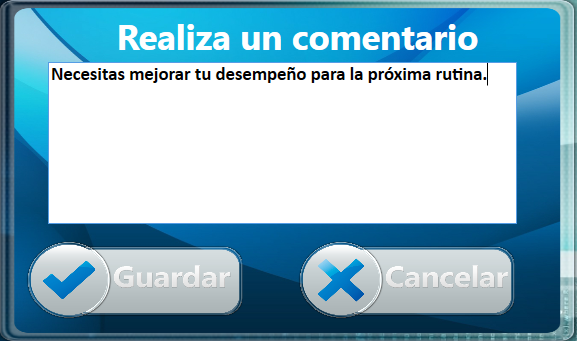
\includegraphics[scale=0.8]{./Figuras/Pantallas/IUE04_4_1Realizar_comentarios}
	\caption{IUE04.4.1 Realizar comentarios}
	\label{fig:IUE04.4.1}
\end{figure}

\textbf{\textcolor[rgb]{0, 0, 0.545098}{Entradas}}\\
En esta pantalla el Entrenador debe capturar la siguiente información:

\begin{itemize}
	\item Un comentario para la rutina seleccionada del Practicante.
\end{itemize}
\vspace{1em}

\textbf{\textcolor[rgb]{0, 0, 0.545098}{Comandos}}
\begin{itemize}
	\item \textbf{\textcolor[rgb]{0, 0, 0.545098}{Guardar:}} Permite al Entrenador registrar o actualizar un comentario acerca de la rutina realizada.
	\item \textbf{\textcolor[rgb]{0, 0, 0.545098}{Cancelar:}} Descarta la información registrada.
\end{itemize}
\vspace{1em}

\textbf{\textcolor[rgb]{0, 0, 0.545098}{Mensajes}}\\
	
\textbf{\nameref{msj:MSG01}}: Se muestra en la pantalla \nameref{pant:IUE04.4.1} cuando se registre un comentario de manera exitosa.\\

\textbf{\nameref{msj:MSG13}}: SSe muestra en la pantalla \nameref{pant:IUE04.4.1} cuando el formato del comentario ingresado por el Entrenador sea incorrecto.\\

\clearpage